%---------------------------------------------------
\chapter{MIDI support} 
\label{midi}
%---------------------------------------------------

Like OSC, several \faust architectures also provide MIDI support. This allows \faust applications to be controlled from any MIDI device (or to control MIDI devices). MIDI is also the preferred way to control polyphonic instruments.

\section{Describing MIDI messages in the DSP source code}

MIDI control messages are described as metadata in UI elements. They are decoded by a special architecture \emph{MidiUI} class that will parse incoming MIDI messages and update the appropriate control parameters, or send MIDI messages when the UI elements (sliders, buttons...) are moved.

\section{Description of the possible standard MIDI messages}

Below, when a 7-bit MIDI parameter is used to drive a button or
checkbox, its maximum value 127 maps to 1 ("on") while its minimum
value 0 maps to 0 ("off").

A special \lstinline'[midi:xxx yyy...]' metadata entry needs to be added to the UI element description. The more usual MIDI messages can be used as described here:

- \lstinline'[midi:ctrl num]' in a slider or bargraph will map the UI element value to (0, 127) range. When used with a button or checkbox, 1 will be mapped to 127, 0 will be mapped to 0,

- \lstinline'[midi:keyon pitch]' in a slider or bargraph will register the UI element's state-variable to be driven by MIDI note-on velocity (an integer between 0 and 127) of the specified key between 0 and 127. When used with a button or checkbox, 1 will be mapped to 127, 0 will be mapped to 0,

- \lstinline'[midi:keyoff pitch]' in a slider or bargraph will register the UI element's state-variable to be driven by MIDI note-off velocity (an integer between 0 and 127) of the specified key between 0 and 127. When used with a button or checkbox, 1 will be mapped to 127, 0 will be mapped to 0,

- \lstinline'[midi:key pitch]' in a slider or bargraph will register the UI element's state-variable to be driven by MIDI note-on velocity (an integer between 0 and 127) of the specified key between 0 and 127. When used with a button or checkbox, 1 will be mapped to 127, 0 will be mapped to 0.  Note-on and note-off events will be handled,

- \lstinline'[midi:keypress pitch]' in a slider or bargraph will register the UI element's state-variable to be driven by the MIDI key-pressure (an integer between 0 and 127) from MIDI key,

- \lstinline'[midi:pgm]' in a slider or nentry will use the UI element range: a received \emph{progchange} value inside this range sets the UI element, and moving the UI element sends the corresponding \emph{progchange} message,

- \lstinline'[midi:chanpress]' in a slider or bargraph will map the UI element value to (0, 127) range, driven by the MIDI channel pressure. When used with a button or checkbox, 1 will be mapped to 127, 0 will be mapped to 0,

- \lstinline'[midi:pitchwheel]' in a slider or bargraph will map the UI element value to (0,16383) range. When used with a button or checkbox, 1 will be mapped to 16383, 0 will be mapped to 0.

\section{MIDI channels}

All the metadata above accept an optional MIDI channel as last parameter, for instance \lstinline'[midi:ctrl 7 2]', \lstinline'[midi:keyon 60 2]' or \lstinline'[midi:pitchwheel 2]'. The UI element then only receives the messages of this channel, and only sends its messages on this channel. Channels are numbered from 1 to 16, and channel 0 (or no channel) means all channels.

A whole program, including its polyphonic voices (see chapter \ref{poly}), can be restricted to a single channel with the \lstinline'[midichannel:n]' option (or the \code{midichannel} metadata):

\begin{lstlisting}
declare options "[midi:on][midichannel:2]";
\end{lstlisting}

Notes, controllers, program change, pressure and pitch-bend messages received on another channel are then ignored. Clock, start, stop and SysEx messages are always received, and the messages sent by the program are not affected. With \lstinline'[midichannel:2]', a UI element declared with \lstinline'[midi:ctrl 7 3]' never receives anything: the channel of a UI element should then be the program channel, or 0.

The standalone applications built with the \code{-midi} option of the \code{faust2xxx} scripts accept a \code{--midi-channel n} parameter at runtime (so using \code{./foo --midi-channel 2} for instance), which takes precedence over the metadata value. Plugin architectures do not apply it, since the host already routes the MIDI channels to each instrument.

\section{A Simple Example}

Here is an example with a \emph{volume} slider controlled with MIDI ctrlchange 7 messages:

\begin{lstlisting}

//-----------------------------------------------
//  Volume MIDI control in dB
//-----------------------------------------------

import("music.lib");

smooth(c) = *(1-c) : +~*(c);
gain = vslider("Volume [midi:ctrl 7]", 0, -70, +4, 0.1) : db2linear : smooth(0.999);
process = *(gain);

\end{lstlisting}

A complete testing example named  \emph{midi\_tester.dsp}  is available in the \faust distribution \emph{examples} folder.

\begin{figure}[h!]
  \centering
  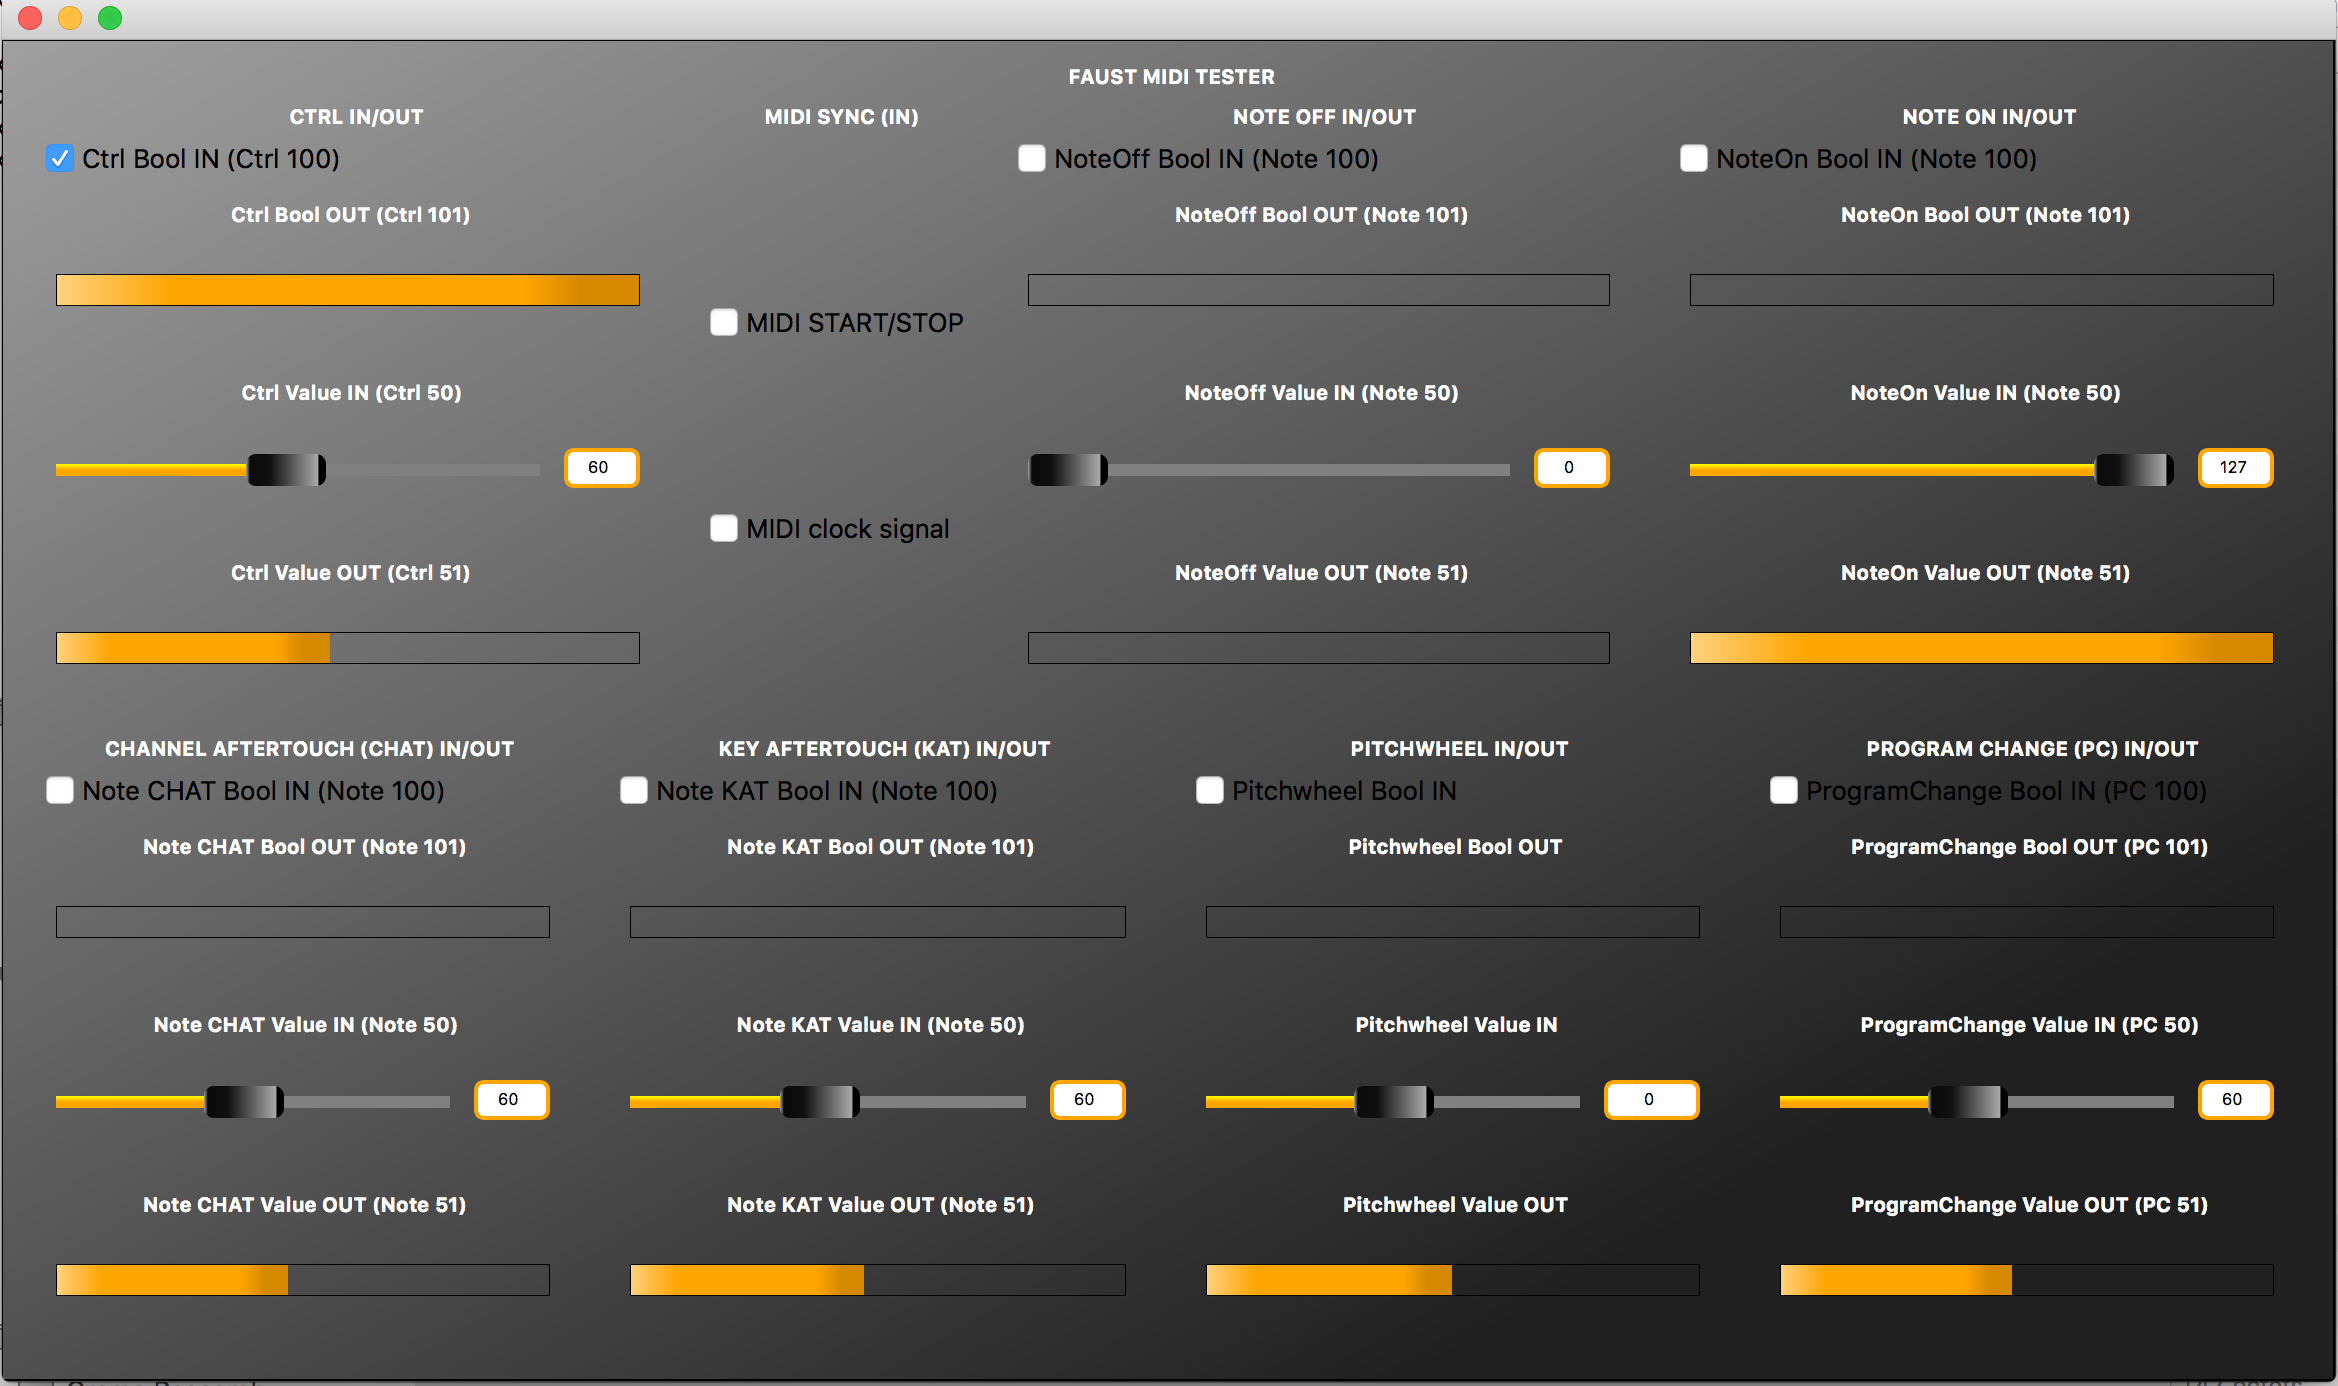
\includegraphics[width=\textwidth]{images/midi-tester.png}
  \caption{MIDI messages testing example}   
  \label{fig:midi-tester}
\end{figure}

MIDI support can be activated using the \code{-midi} option when building the audio application with the appropriate \code{faust2xxx} command. The following table (Table \ref{tab:midiarch}) lists the \faust architectures that provide MIDI support. 

\begin{table}[htp]
\begin{center}
\begin{tabular}{rcc}
\hline
\bf{Audio system} 	& \bf{Environment} & \bf{HTTP support}	\\
\hline
%\OSTab{Linux} \\
%\multicolumn{3}{|l|}{Linux} \\
%\hline
\\
\emph{Linux}\\
Alsa  		& Qt		& yes\\
Jack 			& Qt		& yes\\
%\hline
\\
\emph{Mac OS X} \\
%\hline
CoreAudio 	& Qt 	 & yes\\
Jack 			& Qt  & yes\\
%\hline
\hline
\end{tabular}
\end{center}
\caption{\faust architectures with MIDI support.}
\label{tab:midiarch}
\end{table}

\section{MIDI Synchronization}

MIDI clock-based synchronization can be used to slave a given \faust program. The following three messages need to be used:

- \lstinline'[midi:start]' in a button or checkbox will trigger a value of 1 when a \emph{start} MIDI message is received

- \lstinline'[midi:stop]' in a button or checkbox will trigger a value of 0 when a \emph{stop} MIDI message is received

- \lstinline'[midi:clock]' in a button or checkbox will deliver a sequence of successive 1 and 0 values each time a  \emph{clock} MIDI message is received, seen by \faust code as a square command signal, to be used to compute higher level information.

A typical \faust program will then use the MIDI clock stream to compute the BPM information, or for any synchronization need it may have.  Here is a simple example of a sine wave generated with a frequency controlled by the MIDI clock stream, starting and stopping when receiving the MIDI start/stop messages:

\begin{lstlisting}
import("music.lib");

// square signal (1/0), changing state at each received clock
clocker = checkbox("MIDI clock[midi:clock]");    

// ON/OFF button controlled with MIDI start/stop messages
play = checkbox("ON/OFF [midi:start] [midi:stop]");    

// detect front
front(x) = x != x';     

// count number of peaks during one second
freq(x) = (x-x@SR) : + ~ _;   
   
process = osc(8*freq(front(clocker))) * play;
\end{lstlisting}



